\documentclass{article}
\usepackage{graphicx} % Required for inserting images

\title{Bioinformatics Report}

\begin{document}

\maketitle

\section{Over-expression} %fabio
The first part of the project aims to predict the \textbf{overexpression} of the \textbf{BRCA1} gene. The starting point is feature vectors extracted using \textbf{UNI} from WSI of patients with breast cancer. Using the gene expression associated with our WSIs, we extracted a threshold that we need to construct our dataset. The task is related to a binary classification problem, where elements with a gene expression value below the threshold are assigned the label $0$, while those above are assigned the label $1$. The base models used in our experiments are \textbf{ABMIL} and \textbf{DSMIL}. We also added a model that we called \textbf{DS\_ABMIL}, which replaces the instance classifier of DSMIL with the attention calculation from ABMIL.
All experiments were conducted using a \textbf{Stratified K-fold} with K=5, \textbf{early stopping} with patience=5, 10 epochs, and the \textbf{CosineAnnealingLR} scheduler. All tests were conducted using the same seed to ensure repeatability.

\subsection{ABMIL}
The first model tested is an implementation of ABMIL (cite the paper). First, we apply a linear layer to reduce the input dimensionality from $n\_patch \times 1024$ to a parameter $inner\_dim$. Subsequently, the following attention mechanism is applied:

\begin{equation}
	att = \frac{\exp\{W^\top \tanh(V h^\top) \odot \sigma(U h^\top)\}}{\sum_{j=1}^{n\_patch} \exp\{W^\top \tanh(V h_j^\top) \odot \sigma(U h_j^\top)\}} \quad
\end{equation}

where $U, V \in R^{ n\_patch \times inner\_dim}, w \in R^{n\_patch \times 1}$ are parameters, $\odot$ is an element-wise multiplication, and $\sigma(\cdot)$ is the sigmoid non-linearity.

Subsequently, two linear layers are applied to gradually reduce the dimensionality.
\clearpage
\subsubsection{Results}

In these tests, we focused on studying the performance as the $inner\_dim$ parameter, optimizer, learning rate, and weight decay parameters vary. We observe that the performance of the models remains almost constant despite changes in the hyperparameters. The model tends to always predict class \textbf{"overexprexed"}  because it is the most prevalent. We also note that as the $inner\_dim$ parameter increases, the performance worsens, leading the model to predict only class "overexprexed". In fact, the model with an inner dimension of 128 has a True Positive value of 0.09.

\begin{table}[h]
	\centering
	\begin{tabular}{|ccrc|c|c|c|}
		\hline
		Model & LR & WD & Opt & Accuracy & Precision & Recall\\
		\hline
		ABMIL\_64 & 0,0001 & 0,0001 & AdamW & 0.6868 ± 0.0102 & 0.6955 ± 0.0084 & 0.9418 ± 0.0274 \\
		ABMIL\_64 & 0,0001 & 0,0001 & Radam & 0.6858 ± 0.0082 & 0.6905 ± 0.0099 & 0.9574 ± 0.0215 \\
		ABMIL\_64 & 0,0001 & 0,001 & Radam & 0.6840 ± 0.0089 & 0.6876 ± 0.0102 & 0.9631 ± 0.0243\\
		ABMIL\_64 & 0,0001 & 0,001 & AdamW & 0.6868 ± 0.0102 & 0.6955 ± 0.0084 & 0.9418 ± 0.0274\\
		ABMIL\_128\ & 0,0001 & 0,0001 & AdamW & 0.6792 ± 0.0094 & 0.6812 ± 0.0103 & 0.9745 ± 0.0146 \\
		ABMIL\_32\ & 0,0001 & 0,001 & AdamW & 0.6821 ± 0.0160 & 0.6987 ± 0.0039 & 0.9177 ± 0.0410 \\
		ABMIL\_32\ & 0,0001 & 0,001 & AdamW & 0.6821 ± 0.0160 & 0.6987 ± 0.0039 & 0.9177 ± 0.0410\\
		ABMIL\_32\ & 0,0001 & 0,0001 & Radam & 0.6783 ± 0.0201 & 0.6924 ± 0.0107 & 0.9291 ± 0.0294\\
		ABMIL\_32 & 0,0001 & 0,0001 & Radam & 0.6887 ± 0.0133 & 0.6968 ± 0.0074 & 0.9418 ± 0.0226\\
		\hline
	\end{tabular}
	\centering
	\begin{tabular}{|ccrc|c|c|}
		\hline
		Model & LR & WD & Opt & True Positive & AUC\_ROC\\
		\hline
		ABMIL\_64 & 0,0001 & 0,0001 & AdamW & 0.1803 ± 0.0499 &0.6380 ± 0.0265  \\
		ABMIL\_64 & 0,0001 & 0,0001 & Radam & 0.1465 ± 0.0575& 0.6393 ± 0.0196\\
		ABMIL\_64 & 0,0001 & 0,001 & Radam & 0.1296 ± 0.0600 & 0.6392 ± 0.0198\\
		ABMIL\_64 & 0,0001 & 0,001 & AdamW & 0.1803 ± 0.0499 & 0.6380 ± 0.0265\\
		ABMIL\_128\ & 0,0001 & 0,0001 & AdamW & 0.0930 ± 0.0553&0.6131 ± 0.0121\\
		ABMIL\_32\ & 0,0001 & 0,0001 & AdamW &  0.2141 ± 0.0392&0.6197 ± 0.0122\\
		ABMIL\_32\ & 0,0001 & 0,001 & AdamW & 0.2141 ± 0.0392&0.6196 ± 0.0123\\
		ABMIL\_32\ & 0,0001 & 0,0001 & Radam & 0.1803 ± 0.0422&0.6181 ± 0.0152\\
		ABMIL\_32 & 0,0001 & 0,0001 & Radam & 0.1859 ± 0.0338&0.6203 ± 0.0154\\
		\hline
	\end{tabular}
	\caption{Performances of ABMIL }
\end{table}


\clearpage
\subsection{DSMIL}
The second model we used is DSMIL (cite the paper).As in the previous case, we first applied a linear layer to reduce the dimensionality of our patches.
This model consists of two streams:
\begin{itemize}
	\item The \textbf{instance classifier} is used to extract the critical instance, which is the one with the highest score
	\item The \textbf{bag classifier} is used to create an embedding of the bag based on the similarity of the critical instance with the various instances. Then a bag score is produced
\end{itemize}
The final score of the model is given by the average of the scores from the two streams.

\begin{figure}[h]
	\centering
	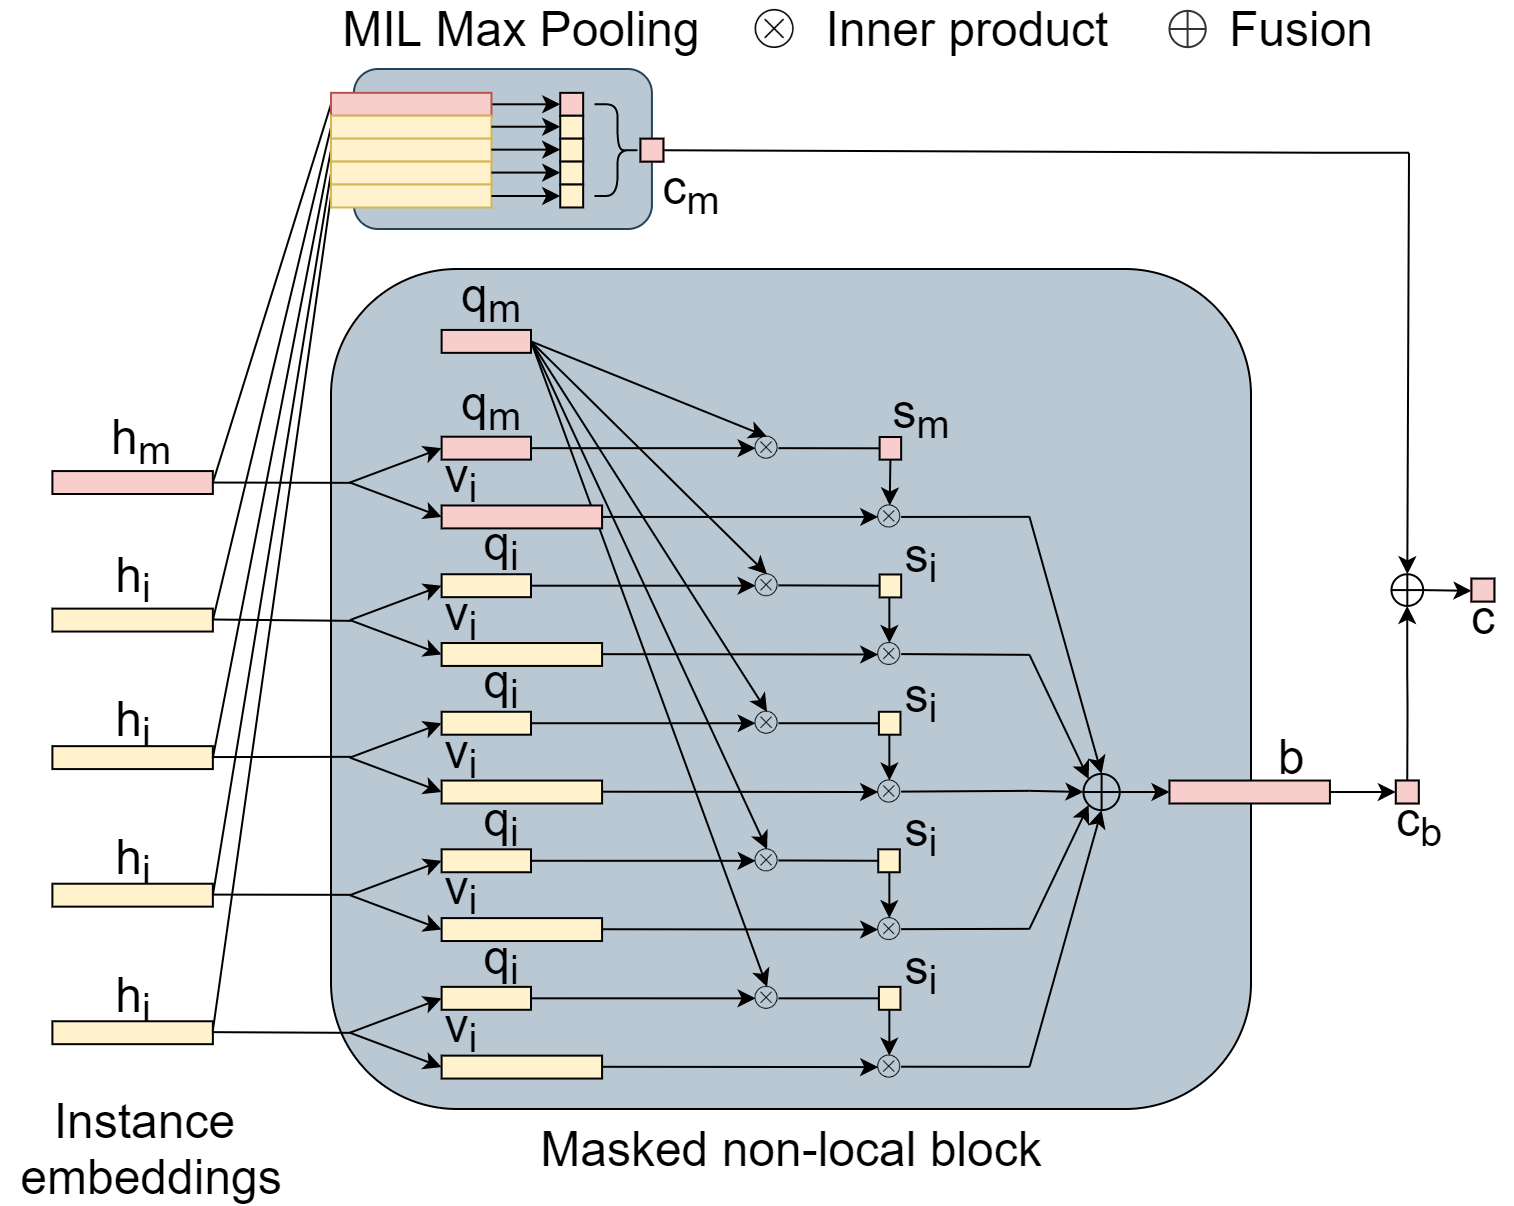
\includegraphics[width=0.8\textwidth]{images/dsmil.png}
	\caption{DSMIL model scheme}
\end{figure}

\clearpage
\subsubsection{Results}
Using a DSMIL, which is a state-of-the-art model for the classification of WSI images, we do not observe improvements compared to what we saw with ABMIL. This is a behavior we have observed every time we increased the number of learnable parameters. As the number of parameters increases, the model progressively loses the ability to distinguish between the two classes and always predicts the most frequent class.

\begin{table}[h]
	\centering
	\begin{tabular}{|ccrc|c|c|c|}
		\hline
		Model & LR & WD & Opt & Accuracy & Precision & Recall \\
		\hline
		DSMIL & 0,0001 & 0,001 & Radam & 0.6962 ± 0.0097 & 0.6958 ± 0.0083 & 0.9660 ± 0.0192 \\
		DSMIL & 0,0001 & 0,001 & AdamW & 0.6764 ± 0.0106 & 0.6871 ± 0.0105 & 0.9447 ± 0.0443 \\
		DSMIL & 0,0001 & 0,0001 & AdamW & 0.6764 ± 0.0106 & 0.6871 ± 0.0105 & 0.9447 ± 0.0443 \\
		DSMIL & 0,0001 & 0,0001 & Radam & 0.6953 ± 0.0082 & 0.6995 ± 0.0073 & 0.9504 ± 0.0185 \\
		\hline
	\end{tabular}
	\centering
	\begin{tabular}{|ccrc|c|c|}
		\hline
		Model & LR & WD & Opt & TP & AUC\_ROC \\
		\hline
		DSMIL & 0,0001 & 0,001 & Radam & 0.1606 ± 0.0433 & 0.6358 ± 0.0144 \\
		DSMIL & 0,0001 & 0,001 & AdamW & 0.1437 ± 0.0779 & 0.6264 ± 0.0144 \\
		DSMIL & 0,0001 & 0,0001 & AdamW & 0.1465 ± 0.0800 & 0.6268 ± 0.0145 \\
		DSMIL & 0,0001 & 0,0001 & Radam & 0.1887 ± 0.0384 & 0.6334 ± 0.0119 \\
		\hline
	\end{tabular}

	\caption{Performance on DSMIL}
\end{table}

\clearpage

\subsection{DS\_ABMIL}
This model is our proposal and has the same two-stream structure as DSMIL. The instance classifier is replaced by the attention calculation of ABMIL. The critical patch is extracted through max pooling on the attention scores.

\subsubsection{Results}

Contrary to what was observed in the previous experiments, the results we obtain are not influenced by the choice of hyperparameters, the optimizer, or the internal dimensionality used.
This is the only case in which a slight increase in the number of parameters leads to an improvement in performance.

\begin{table}[h]
	\centering
	\begin{tabular}{|ccrc|c|c|c|}
		\hline
		Modello & LR & WD & Opt & Accuracy & Precision & Recall \\
		\hline
		DS\_ABMIL\_128 & 0,0001 & 0,001 & Radam & 0.6604 ± 0.0244 & 0.7007 ± 0.0152 & 0.8553 ± 0.0463 \\
		DS\_ABMIL\_128 & 0,0001 & 0,001 & AdamW & 0.6632 ± 0.0236 & 0.6966 ± 0.0148 & 0.8752 ± 0.0405 \\
		DS\_ABMIL\_128 & 0,0001 & 0,0001 & AdamW & 0.6660 ± 0.0282 & 0.6968 ± 0.0166 & 0.8823 ± 0.0517 \\
		DS\_ABMIL\_128 & 0,0001 & 0,0001 & Radam & 0.6736 ± 0.0096 & 0.7002 ± 0.0052 & 0.8908 ± 0.0227 \\
		DS\_ABMIL\_32 & 0,0001 & 0,0001 & AdamW & 0.6840 ± 0.0089 & 0.6953 ± 0.0159 & 0.9376 ± 0.0368 \\
		DS\_ABMIL\_32 & 0,0001 & 0,0001 & Radam & 0.6821 ± 0.0110 & 0.7024 ± 0.0117 & 0.9078 ± 0.0426 \\
		DS\_ABMIL\_32 & 0,0001 & 0,001 & Radam & 0.6755 ± 0.0069 & 0.6848 ± 0.0136 & 0.9518 ± 0.0419 \\
		DS\_ABMIL\_32 & 0,0001 & 0,001 & AdamW & 0.6821 ± 0.0102 & 0.7028 ± 0.0122 & 0.9064 ± 0.0384 \\
		DS\_ABMIL\_64 & 0,0001 & 0,001 & AdamW & 0.6745 ± 0.0181 & 0.6991 ± 0.0037 & 0.8965 ± 0.0470 \\
		DS\_ABMIL\_64 & 0,0001 & 0,0001 & AdamW & 0.6726 ± 0.0170 & 0.6936 ± 0.0149 & 0.9135 ± 0.0658 \\
		DS\_ABMIL\_64 & 0,0001 & 0,001 & Radam & 0.6764 ± 0.0240 & 0.6980 ± 0.0142 & 0.9064 ± 0.0518\\
		DS\_ABMIL\_64 & 0,0001 & 0,0001 & Radam	&0.6726 ± 0.0077 & 0.6965 ± 0.0127 & 0.9035 ± 0.0594 \\
		\hline
	\end{tabular}
	\begin{tabular}{|ccrc|c|c|}
		\hline
		Model & LR & WD & Opt & TP & AUC\_ROC \\
		\hline
		DS\_ABMIL\_128 & 0,0001 & 0,001 & Radam & 0.2732 ± 0.0640 & 0.6378 ± 0.0201 \\
		DS\_ABMIL\_128 & 0,0001 & 0,001 & AdamW & 0.2423 ± 0.0594 & 0.6285 ± 0.0203 \\
		DS\_ABMIL\_128 & 0,0001 & 0,0001 & AdamW & 0.2366 ± 0.0681 & 0.6330 ± 0.0210 \\
		DS\_ABMIL\_128 & 0,0001 & 0,0001 & Radam & 0.2423 ± 0.0287 & 0.6314 ± 0.0108 \\
		DS\_ABMIL\_32 & 0,0001 & 0,0001 & AdamW & 0.1803 ± 0.0901 & 0.6283 ± 0.0161 \\
		DS\_ABMIL\_32 & 0,0001 & 0,0001 & Radam & 0.2338 ± 0.0732 & 0.6362 ± 0.0222 \\
		DS\_ABMIL\_32 & 0,0001 & 0,001 & Radam & 0.1268 ± 0.0904 & 0.6383 ± 0.0113 \\
		DS\_ABMIL\_32 & 0,0001 & 0,001 & AdamW & 0.2366 ± 0.0737 & 0.6210 ± 0.0178 \\
		DS\_ABMIL\_64 & 0,0001 & 0,001 & AdamW & 0.2338 ± 0.0433 & 0.6331 ± 0.0154 \\
		DS\_ABMIL\_64 & 0,0001 & 0,0001 & AdamW & 0.1944 ± 0.1089 & 0.6405 ± 0.0109\\
		DS\_ABMIL\_64 & 0,0001 & 0,001 & Radam & 0.2197 ± 0.0748 & 0.6359 ± 0.0248\\
		DS\_ABMIL\_64 & 0,0001 & 0,0001 & Radam	& 0.2141 ± 0.0973 & 0.6302 ± 0.0190\\
		\hline
	\end{tabular}

	\caption{Performances on DS\_ABMIL}
\end{table}
\clearpage
\subsection{Regression Approach}
Another approach we attempted was to view the problem as a regression. The goal was to predict the value of the BRCA1 gene. We conducted tests with ABMIL and DS\_ABMIL, but the results obtained were not satisfactory.

\begin{table}[h]
	\centering
	\begin{tabular}{|ccrc|c|c|c|}
		\hline
		Model & LR & WD & Opt & MAE & MSE & R2 \\ 
		\hline
		AB\_MIL & 0.001 & 0.001 & AdamW & 4.4387 ± 0.2252 & 34.6050 ± 1.0267 & 0.0677 ± 0.0277 \\
		DS\_ABMIL & 0.001 & 0.001 & AdamW & 4.4001 ± 0.2568 & 35.4324± 1.1058 & 0.0454 ± 0.0298 \\ 
		\hline
	\end{tabular}
 \caption{Results on regression task}
\end{table}

\subsection{Comparison}

In this section, we will compare the performance of the tested models. The performance we obtain is consistent across all three models. The \textbf{DS\_ABMIL} model we created has proven to be more robust to variations in hyperparameters and provides the best performances. All the models we tested have difficulty correctly classifying the $underexpressed$ class. We also observe that increasing the number of parameters in our models or testing other models with a significant number of parameters yields worse results. This behavior is caused by the reduced dimensionality of our dataset.


\begin{table}[h]
	\centering
	\begin{tabular}{|ccrc|c|c|c|}
		\hline
		Modello & LR & WD & Opt & Accuracy & Precision & Recall \\
		\hline
		ABMIL\_32\ & 0,0001 & 0,001 & AdamW & 0.6821 ± 0.0160 & 0.6987 ± 0.0039 & 0.9177 ± 0.0410 \\
		DSMIL & 0,0001 & 0,0001 & Radam & 0.6953 ± 0.0082 & 0.6995 ± 0.0073 & 0.9504 ± 0.0185 \\
		DS\_ABMIL\_128 & 0,0001 & 0,001 & Radam & 0.6604 ± 0.0244 & 0.7007 ± 0.0152 & 0.8553 ± 0.0463 \\
		DS\_ABMIL\_32 & 0,0001 & 0,001 & AdamW & 0.6821 ± 0.0102 & 0.7028 ± 0.0122 & 0.9064 ± 0.0384 \\
		\hline
	\end{tabular}
	\begin{tabular}{|ccrc|c|c|}
		\hline
		Model & LR & WD & Opt & TP & AUC\_ROC \\
		\hline
		ABMIL\_32\ & 0,0001 & 0,001 & AdamW & 0.2141 ± 0.0392&0.6196 ± 0.0123\\
		DSMIL & 0,0001 & 0,0001 & Radam & 0.1887 ± 0.0384 & 0.6334 ± 0.0119 \\
		DS\_ABMIL\_128 & 0,0001 & 0,001 & Radam & 0.2732 ± 0.0640 & 0.6378 ± 0.0201 \\
		DS\_ABMIL\_32 & 0,0001 & 0,001 & AdamW & 0.2366 ± 0.0737 & 0.6210 ± 0.0178 \\
		\hline
	\end{tabular}
	
	\caption{Performances comparison}
\end{table}





\clearpage
\section{Attention Map} %fabio
The ultimate goal of our project is to visualize attention maps that provide an explanation for the decisions made by the model. The models we tested utilize whole slide images (WSI) represented through UNI features with a shape of $n\_patch\times1024$. What we have done is overlay a heat-map representing the importance of each patch onto a reduced version of the WSI.
This process is composed by two steps:
\begin{itemize}
	\item compute the attention on the single patch
	\item compute the activation map of each patch
\end{itemize}

Add block scheme

\subsection{Patch-level attention}

Starting from the identifier of a WSI, we can input it into our model to obtain the desired classification as well as the attention for each individual patch. The attention scores are normalized and overlaid onto a reduced version of the WSI to identify which patches are the most important.

\begin{figure}[h]
	\centering
	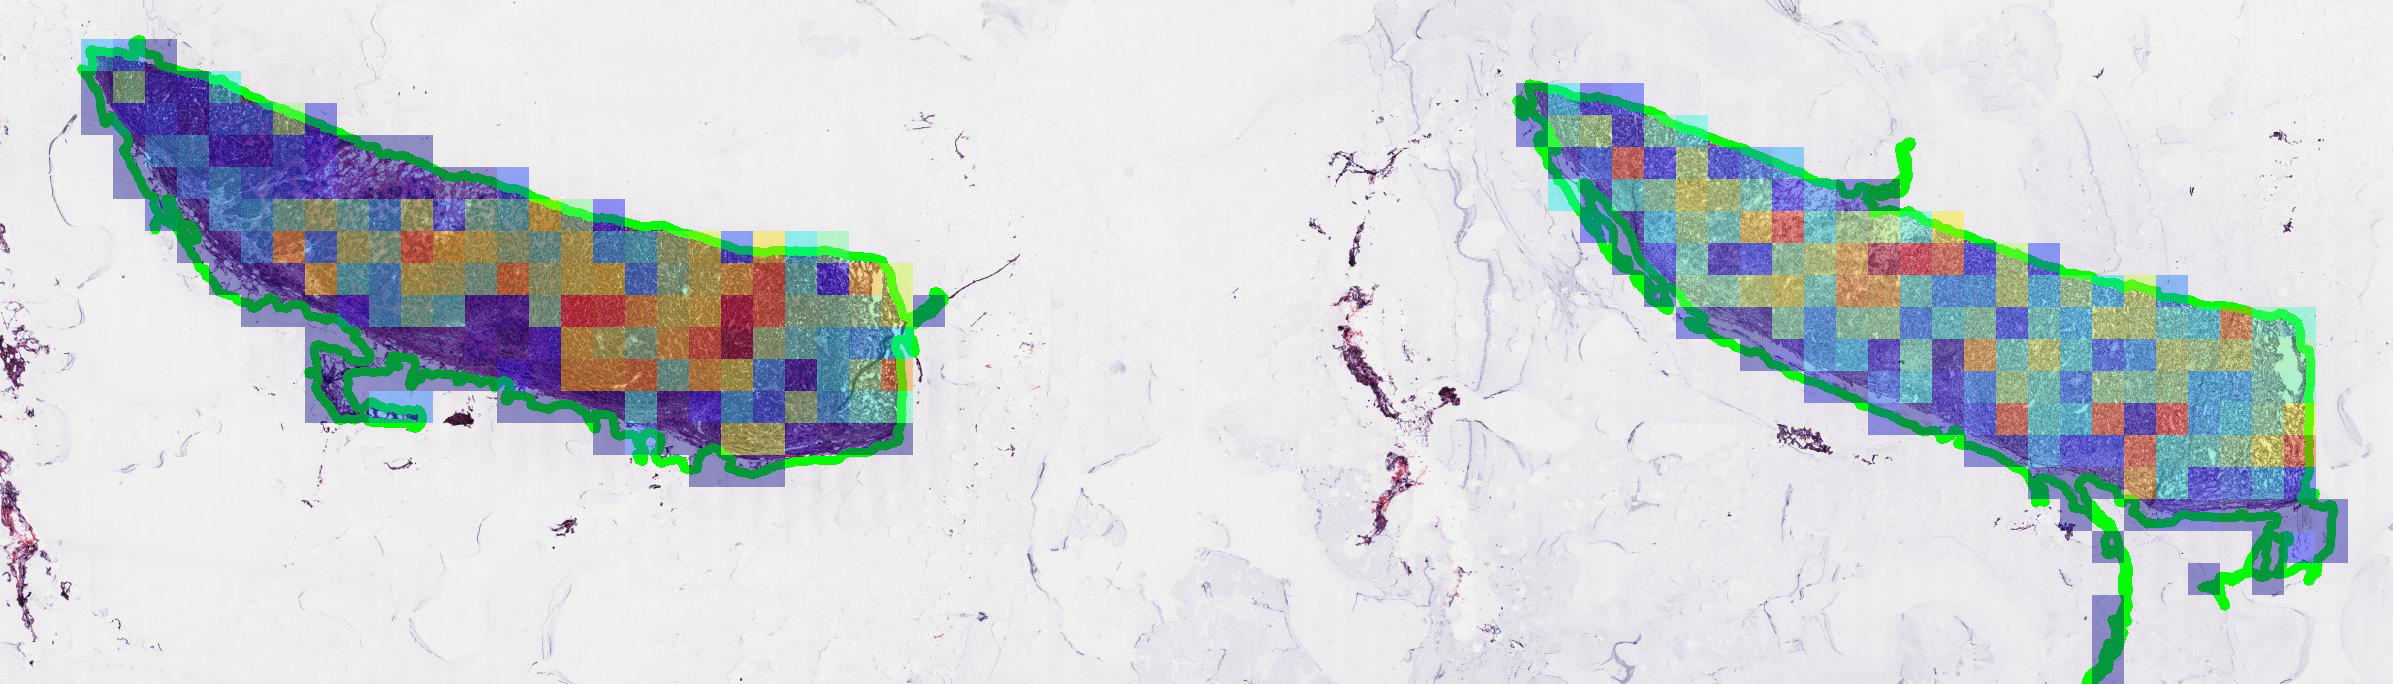
\includegraphics[width=1\textwidth]{images/old_attention_map_val.png}
	\caption{Patch-level attention projected on to the WSI. Warmer colors means higher importance}
\end{figure}


\subsection{Inner patch attivation}
We have introduced this step to obtain an attention map that also considers the importance of the elements within each individual patch. Each patch, which has a size of $1024\times1024$, is resized to $224\times224$ and subsequently passed through a ResNet50. This is done to obtain the activation map.

For each patch, we multiply the normalized activation map by the normalized attention value obtained in the previous step. In this way, we generate a heat-map to overlay on the image that takes into account both the importance of the patch in the decision of our model and the internal features of each patch.

Before being utilized, we applied a Gaussian filter with $\sigma =2$ to smooth the edges between the patches. Additionally, a threshold was applied to display only values that had scores exceeding $0.8$.
 
\begin{figure}[h]
	\centering
	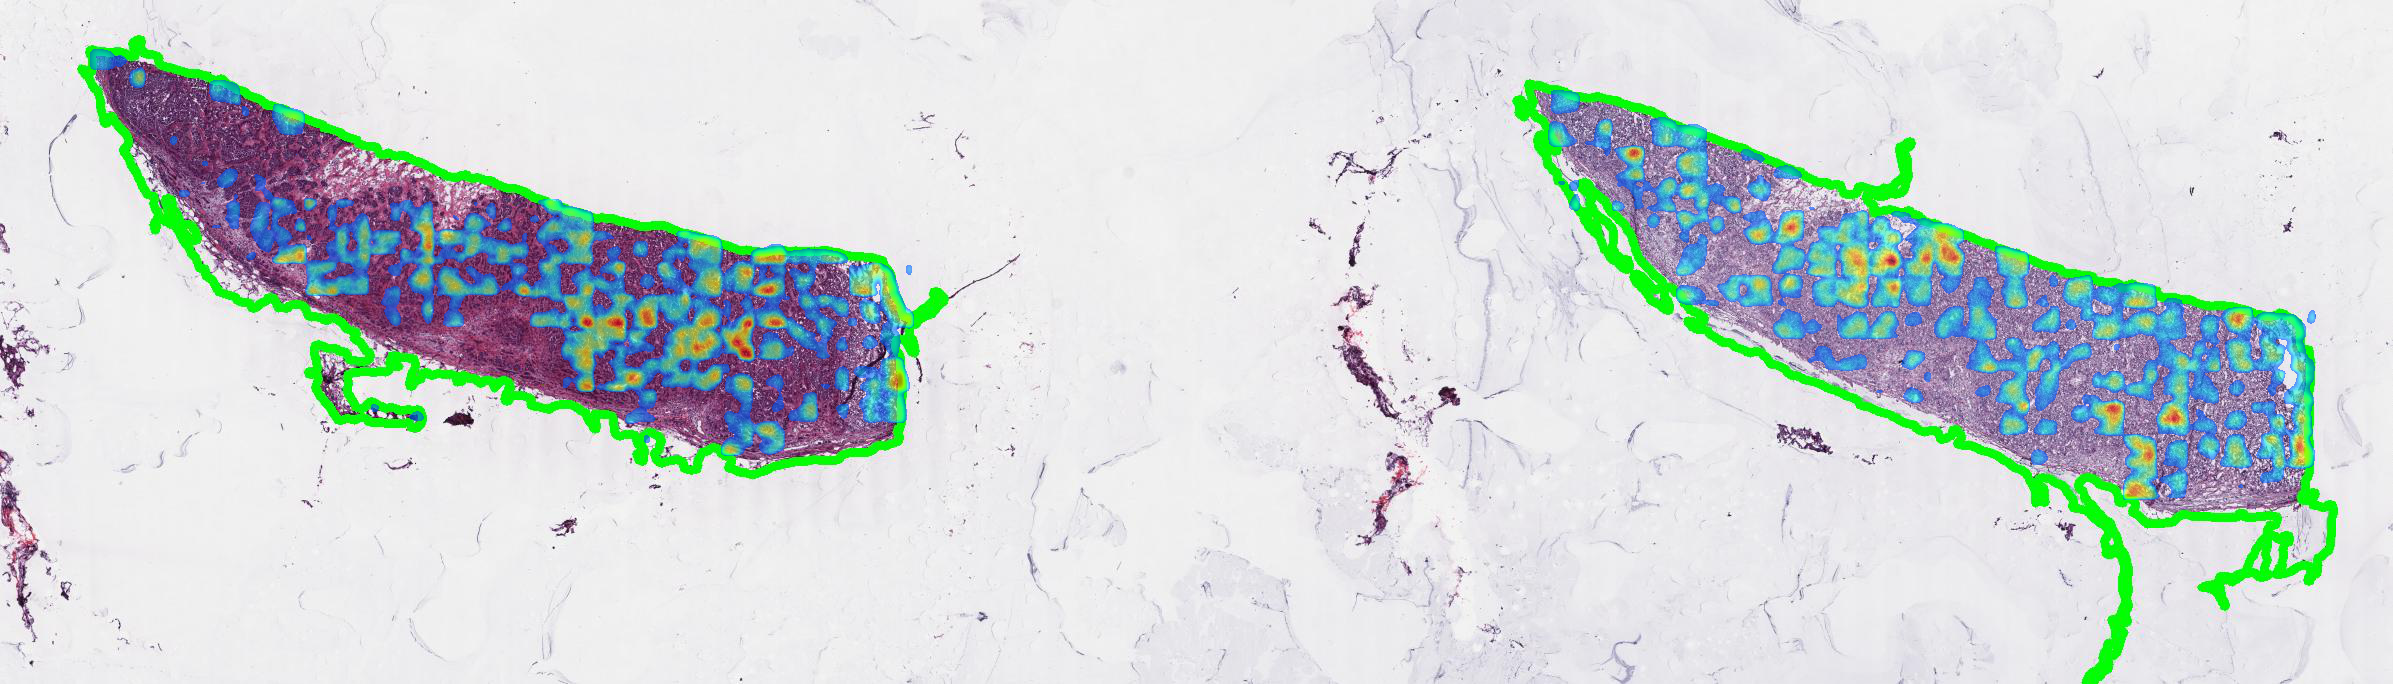
\includegraphics[width=1\textwidth]{images/attention_map_val.png}
	\caption{Final result that takes into account patch-level attention and inner patch features}
\end{figure}

\newpage

\end{document}